% CREATED BY DAVID FRISK, 2014

% COVER PAGE
\begin{titlepage}
\newgeometry{top=3cm, bottom=3cm,
			left=2.25 cm, right=2.25cm}	% Temporarily change margins		
			
% Cover page background 
\AddToShipoutPicture*{\backgroundpic{-4}{56.7}{figure/auxiliary/frontpage_gu_eng.pdf}}
\addtolength{\voffset}{2cm}

% Cover picture (replace with your own or delete)		
%\begin{figure}[h!]
%\centering
%\vspace{2cm}	% Adjust vertical spacing here
%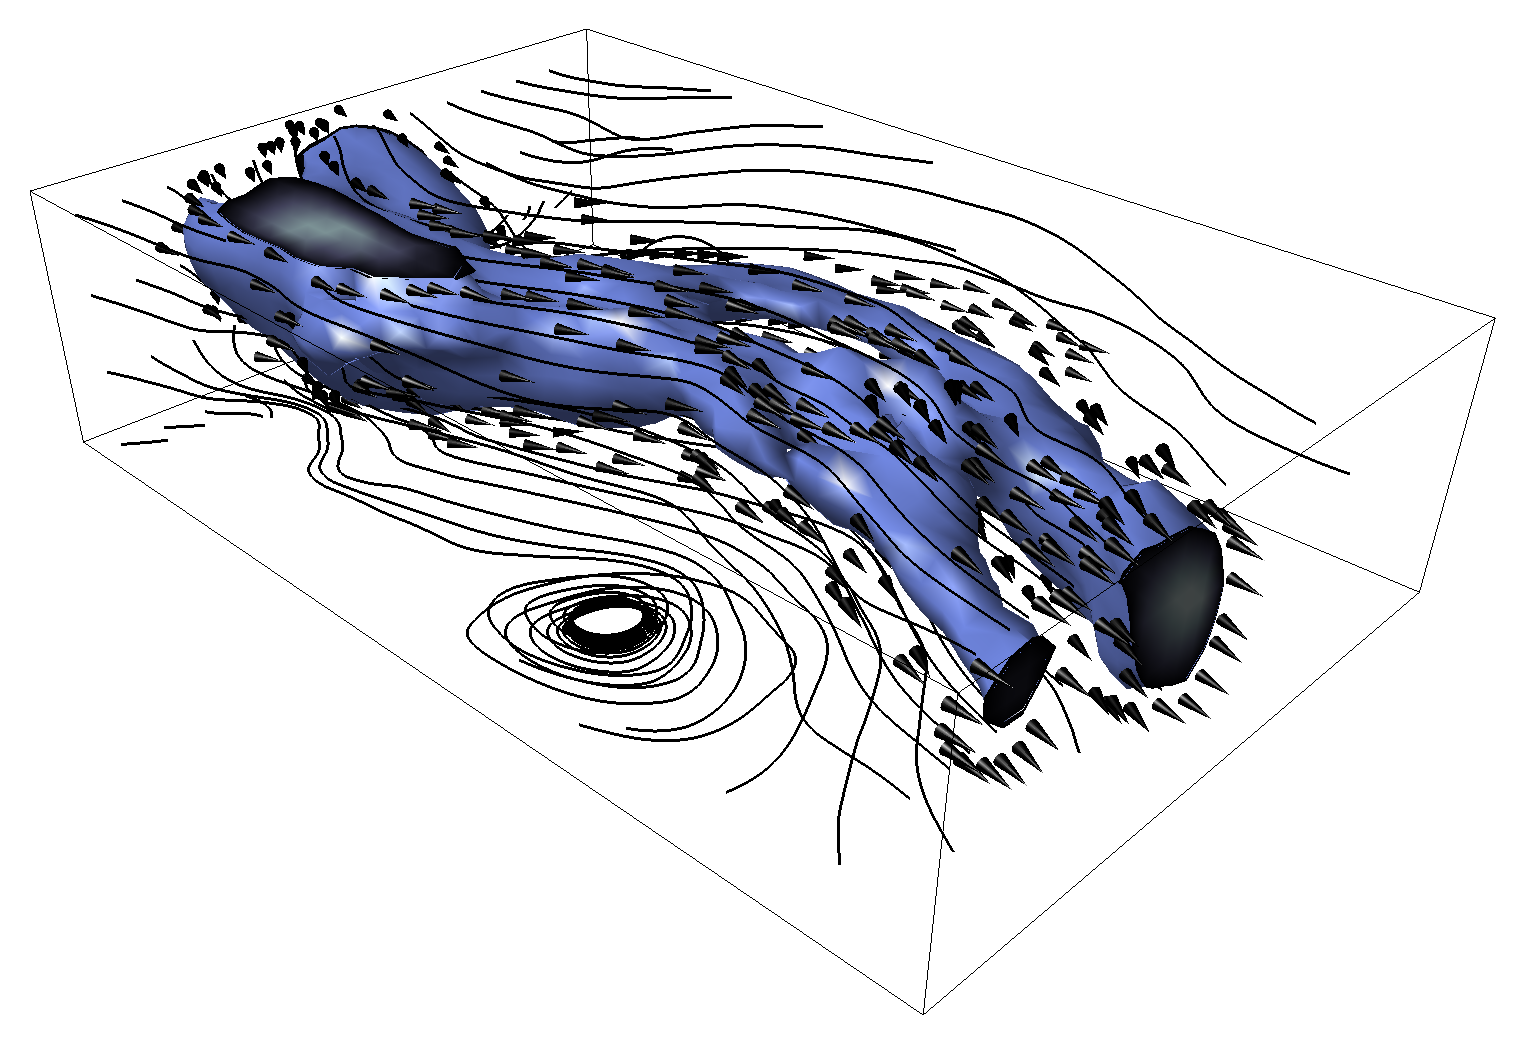
\includegraphics[width=0.9\linewidth]{figure/Wind.png}
%\end{figure}

% Cover text
\mbox{}
\vfill
\renewcommand{\familydefault}{\sfdefault} \normalfont % Set cover page font
\textbf{{\Huge	The Hopper language 	\\[0.2cm] 
				}} 	\\[0.5cm]
{\Large A Haskell-like language on the Erlang VM}\\[0.5cm]
Bachelor of Science Thesis in Computer Science and Engineering \\[0.5cm]

{\Large
\todo{Alfabetical order}
  William Hughes \\
  Björn Norgren \\
  David Lindbom \\
  Jakob Jarmar   \\
  Johan Larsson \\
  David Lindbom \\
  Björn Norgren \\
  Johan Wikström Schützer \\
  }\\[2.0cm]


Department of Computer Science and Engineering \\
\textsc{Chalmers University of Technology} \\
\textsc{University of Gothenburg} \\
Gothenburg, Sweden, Spring 2015

\renewcommand{\familydefault}{\rmdefault} \normalfont % Reset standard font
\end{titlepage}


% BACK OF COVER PAGE (BLANK PAGE)
\newpage
\restoregeometry
\thispagestyle{empty}
\mbox{}


%% TITLE PAGE
%\newpage
%\thispagestyle{empty}
%\begin{center}
%	\textsc{\large DATX02-15-29}\\[4cm]
%	\textbf{\Large The Hopper Language} \\[1cm]
%	{\large A Haskell-like language on the Erlang VM}\\[1cm]
%  {\Large William Hughes \\
%          Jakob Jarmar   \\
%          Johan Larsson \\
%          David Lindbom \\
%          Björn Norgren \\
%          Johan Wikström Schützer }\\[2.0cm]
%	
%	\vfill	
%	% Logotype on titlepage	
%	\begin{figure}[h!]
%	\centering
%	% Remove the following line to remove the titlepage logotype
%        \subfloat{
\includegraphics[width=0.2\pdfpagewidth]{figure/auxiliary/logo_eng.pdf}}
%        \subfloat{
\includegraphics[width=0.2\pdfpagewidth]{figure/auxiliary/logo_gu_eng.eps}} \\	
%	\end{figure}	\vspace{5mm}	
%	
%	Department of Computer Science and Engineering \\
%	%\emph{Division of Division name}\\
%	DATX02-15-29\\
%	\textsc{Chalmers University of Technology} \\
%	\textsc{University of Gothenburg} \\
%	Gothenburg, Sweden, Spring 2015 \\
%\end{center}


% IMPRINT PAGE (BACK OF TITLE PAGE)
\newpage
\thispagestyle{plain}
\vspace*{4.5cm}
The Hopper Language\\
A Haskell-like language on the Erlang VM\\
William Hughes \\
Jakob Jarmar   \\
Johan Larsson \\
David Lindbom \\
Björn Norgren \\
Johan Wikström Schützer \\[0.5cm]

\copyright ~ William Hughes, 2015.\\
\copyright ~ Jakob Jarmar, 2015.\\
\copyright ~ Johan Larsson, 2015.\\
\copyright ~ David Lindbom, 2015.\\
\copyright ~ Björn Norgren, 2015.\\
\copyright ~ Johan Wikström Schützer, 2015.\\[0.5cm]

Supervisor: Nicholas Smallbone, Department of Computer Science and Engineering\\
Examiner: Arne Linde, Department of Computer Science and Engineering\\[0.5cm]

Bachelor Thesis 2015:29\\
Department of Computer Science and Engineering\\
%Division of Division name\\
DATX02-15-29\\
Chalmers University of Technology\\
University of Gothenburg\\
SE-412 96 Gothenburg\\
Telephone +46 31 772 1000\\

\vfill
% Caption for cover page figure if used, possibly with reference to further information in the report
%Cover: Wind visualization constructed in Matlab showing a surface of constant wind speed along with streamlines of the flow. \\

Typeset in \LaTeX \\
%Printed by [Name of printing company]\\
Gothenburg, Sweden 2015
